\chapter{Introduction to Probability}

\section{What is probability?}

Probability is the mathematical language for \emph{uncertainty}. Whenever we perform an
experiment whose outcome cannot be predicted with certainty (flipping a coin, measuring
the lifetime of a light bulb, counting the number of emails that arrive in an hour) we
would like a number between $0$ and $1$ that measures how likely each possible outcome is.

Stat 230 builds the theory of probability from a small set of axioms and then develops
the standard models (binomial, Poisson, normal, \dots) that are used throughout
statistics (Stat 231), actuarial science and computer science. Before the axioms, it is
worth asking what a probability actually \emph{means}. There are three classical
interpretations.

\subsection{The classical definition}

\begin{definition}[Classical probability]
If an experiment has a finite number of possible outcomes, all of which are \emph{equally
likely}, then the probability of an event $A$ is
\[
  P(A) = \frac{\text{number of outcomes in } A}{\text{total number of outcomes}}.
\]
\end{definition}

\begin{example}
Roll a fair six-sided die. The probability of an even number is $3/6 = 1/2$, since three
of the six equally likely faces ($2,4,6$) are even.
\end{example}

\textbf{Limitations.} The definition is circular (``equally likely'' already means
``equally probable''), and it only applies when the outcomes really are symmetric. It
says nothing about a biased coin, or about the probability that it rains tomorrow.

\subsection{The relative frequency definition}

\begin{definition}[Relative frequency probability]
The probability of an event $A$ is the limiting proportion of times $A$ occurs when the
experiment is repeated a very large number of times under identical conditions:
\[
  P(A) = \lim_{n\to\infty} \frac{\text{number of times $A$ occurs in $n$ trials}}{n}.
\]
\end{definition}

\begin{example}
A thumbtack is tossed $1000$ times and lands point-up $612$ times. The relative frequency
estimate of $P(\text{point up})$ is $0.612$. There is no symmetry argument available
here, so the classical definition is useless.
\end{example}

\textbf{Limitations.} We can never actually perform infinitely many trials, and many
experiments cannot be repeated at all (``Will this particular startup succeed?'').

\subsection{The subjective definition}

\begin{definition}[Subjective probability]
The probability of an event is a measure of how strongly a particular person believes the
event will occur, often calibrated by the odds at which they would be willing to bet on
it.
\end{definition}

\begin{example}
A sports analyst says the Raptors have a $30\%$ chance of winning the title this year.
This is a statement about the analyst's degree of belief; another analyst may give a
different number.
\end{example}

\textbf{Limitations.} Different people get different answers, so this is hard to use as an
objective scientific foundation, although it is the starting point of Bayesian
statistics.

\begin{important}[The modern approach]
None of the three definitions is fully satisfactory, so Stat 230 takes a
\emph{mathematical} approach: we write down a \emph{probability model} (a sample space and
a function $P$ satisfying a few axioms, Chapter 2) and derive consequences. Any of the
three interpretations can then be used to decide which model is appropriate for a real
situation.
\end{important}

\section{Sample spaces}

\begin{definition}[Experiment, sample space]
An \emph{experiment} is any procedure that can be repeated (at least in principle) and has
a well-defined set of possible outcomes. A \emph{sample space} $S$ is a set of possible
outcomes such that every run of the experiment produces exactly one element of $S$.
\end{definition}

The sample space is not unique: it depends on what we decide to record.

\begin{example}[Different sample spaces for the same experiment]
Roll a die twice.
\begin{itemize}
  \item If we record the ordered pair of faces,
        $S_1 = \{(i,j) : i,j \in \{1,\dots,6\}\}$, which has $36$ outcomes.
  \item If we only record the sum, $S_2 = \{2,3,\dots,12\}$, which has $11$ outcomes.
\end{itemize}
The outcomes of $S_1$ are equally likely for fair dice; those of $S_2$ are not (a sum of
$7$ arises in $6$ ways, a sum of $2$ in only one). Choosing a sample space with equally
likely outcomes often makes calculations much easier.
\end{example}

\begin{definition}[Discrete sample space]
A sample space is \emph{discrete} if it is finite or countably infinite (its elements can
be listed $a_1, a_2, a_3, \dots$). Otherwise (e.g.\ an interval of real numbers) it is
\emph{non-discrete} or \emph{continuous}.
\end{definition}

\begin{example}
Two experiments with very different sample spaces:
\begin{itemize}
  \item Toss a coin until the first head appears and record the number of tosses:
        $S = \{1,2,3,\dots\}$ is countably infinite, hence discrete.
  \item Measure the time (in hours) until a bulb burns out: $S = [0,\infty)$, which is
        not discrete.
\end{itemize}
\end{example}

The first part of the course works with discrete sample spaces; continuous models appear
in Chapter 7.

\section{Events}

\begin{definition}[Event]
An \emph{event} is a subset $A \subseteq S$ of the sample space. We say $A$
\emph{occurs} if the outcome of the experiment is an element of $A$. An event containing a
single outcome is a \emph{simple event}; an event with more than one outcome is a
\emph{compound event}.
\end{definition}

\begin{example}
For two rolls of a die with $S_1$ as above, the event ``the sum is $4$'' is
\[
  A = \{(1,3),(2,2),(3,1)\},
\]
a compound event made of three simple events.
\end{example}

Since events are sets, we combine them using set operations. Let $A, B \subseteq S$.

\begin{center}
\begin{tabular}{lll}
\toprule
Notation & Name & Occurs when \\
\midrule
$A \cup B$ & union & at least one of $A$, $B$ occurs \\
$A \cap B$ (also $AB$) & intersection & both $A$ and $B$ occur \\
$\bar A$ (also $A^c$) & complement & $A$ does not occur \\
$\emptyset$ & null event & never \\
$S$ & certain event & always \\
\bottomrule
\end{tabular}
\end{center}

\begin{definition}[Mutually exclusive]
Events $A$ and $B$ are \emph{mutually exclusive} (or \emph{disjoint}) if
$A \cap B = \emptyset$, i.e.\ they cannot both occur.
\end{definition}

\subsection{Venn diagrams and De Morgan's laws}

\begin{center}
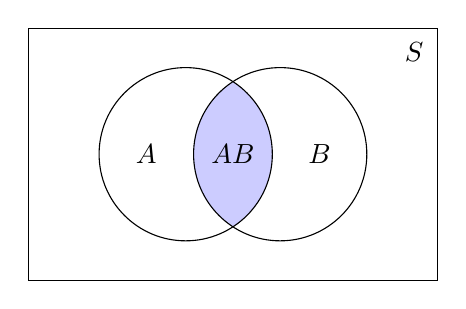
\begin{tikzpicture}
  \draw (-2.6,-1.6) rectangle (2.6,1.6);
  \node at (2.3,1.3) {$S$};
  \begin{scope}
    \clip (-0.6,0) circle (1.1);
    \fill[blue!20] (0.6,0) circle (1.1);
  \end{scope}
  \draw (-0.6,0) circle (1.1);
  \draw (0.6,0) circle (1.1);
  \node at (-1.1,0) {$A$};
  \node at (1.1,0) {$B$};
  \node at (0,0) {$AB$};
\end{tikzpicture}
\end{center}

Venn diagrams are useful for guessing identities, but proofs should use the definitions.
The most useful identities are:

\begin{theorem}[De Morgan's laws]
For any events $A$ and $B$,
\[
  \overline{A\cup B} = \bar A \cap \bar B, \qquad \overline{A \cap B} = \bar A \cup \bar B.
\]
\end{theorem}

\begin{proof}
An outcome is in $\overline{A\cup B}$ iff it is in neither $A$ nor $B$, iff it is in both
$\bar A$ and $\bar B$. The second law follows by applying the first to $\bar A$, $\bar B$
and taking complements.
\end{proof}

Other standard rules: union and intersection are commutative and associative, and each
distributes over the other:
$A \cap (B \cup C) = (A\cap B)\cup(A \cap C)$ and $A \cup (B\cap C) = (A\cup B)\cap(A\cup C)$.

\begin{example}
In words, ``not (rain or snow)'' is the same as ``no rain and no snow''. If $A$ is the event
that a randomly chosen student takes Stat 230 and $B$ the event that they take Math 239,
then $\bar A \cap \bar B$ (``takes neither'') is the complement of $A \cup B$ (``takes at
least one'').
\end{example}

\section{Assigning probabilities in a discrete sample space}

For a discrete sample space $S = \{a_1, a_2, \dots\}$ we assign to each simple event a
number $P(a_i)$ with
\[
  0 \le P(a_i) \le 1 \quad\text{and}\quad \sum_{i} P(a_i) = 1,
\]
and then define, for any event $A$,
\[
  P(A) = \sum_{a_i \in A} P(a_i).
\]
This set of numbers is called a \emph{probability distribution} on $S$. The rules are
consistent with all three interpretations above.

\begin{example}[Two dice]
With $S_1$ and fair dice, each of the $36$ outcomes has probability $1/36$. The
probability that the sum is $7$ is
\[
  P(\{(1,6),(2,5),(3,4),(4,3),(5,2),(6,1)\}) = \frac{6}{36} = \frac16,
\]
and the probability that the sum is $4$ is $3/36 = 1/12$.
\end{example}

\begin{example}[Countably infinite $S$]
Toss a fair coin until the first head and let $S=\{1,2,\dots\}$ be the number of tosses.
The first head occurs on toss $k$ exactly when the first $k-1$ tosses are tails and the
$k$th is a head, so $P(k) = (1/2)^k$. These are valid probabilities since
\[
  \sum_{k=1}^\infty \left(\tfrac12\right)^k = \frac{1/2}{1-1/2} = 1.
\]
The probability that more than $3$ tosses are needed is
$1 - (1/2 + 1/4 + 1/8) = 1/8$, which also equals the probability that the first three
tosses are all tails.
\end{example}

\begin{important}[Common pitfall]
Do not assume outcomes are equally likely just because the sample space is finite. In
$S_2=\{2,\dots,12\}$ (sum of two dice) the outcome $7$ has probability $6/36$, not
$1/11$. Always ask whether there is a symmetry that justifies equal probabilities.
\end{important}

\section{Summary}

\begin{itemize}
  \item Three interpretations of probability: classical (equally likely outcomes),
        relative frequency (long-run proportion), subjective (degree of belief).
  \item A sample space $S$ lists the possible outcomes; it is discrete if finite or
        countably infinite. The same experiment can have several sample spaces.
  \item Events are subsets of $S$, combined with $\cup$, $\cap$ and complements;
        De Morgan's laws convert between them.
  \item On a discrete $S$, a probability distribution assigns non-negative numbers
        summing to $1$ to the outcomes, and $P(A)$ is the sum over the outcomes in $A$.
\end{itemize}
